\ifx\allfiles\undefined
%生成目录超链接，使用UTF8字符集
\documentclass[12pt,UTF8]{ctexart}


\usepackage{mathtools}%花括号括起的公式
\usepackage{enumerate}%列表
\usepackage{graphicx}%表格
\usepackage[table]{xcolor}%彩色表格
\usepackage{booktabs}%调整表格行高


\renewcommand\tabcolsep{50pt}
\renewcommand\arraystretch{2}

%文本框
\usepackage{tcolorbox}
\tcbuselibrary{skins,vignette,raster,listings,listingsutf8,theorems, breakable,magazine,fitting}

%页面设置
\usepackage{geometry}%设置页面
\usepackage{setspace}%设置局部行距

\usepackage{ctex}
\usepackage{CJK}

%图像处理
\usepackage{graphicx}
\usepackage{float}%允许浮动
\usepackage{caption}%设置标题
\usepackage{graphicx, subfig}

%附录
\usepackage[toc,page]{appendix}

%导言区
\title{中小微企业的信贷决策}

%不要页眉
\pagestyle{plain}
\bibliographystyle{plain}

\geometry{a4paper}%将纸张设置为A4大小

%修改文档结构层次的名称
\usepackage{titlesec}%chapter1修改为一
\titleformat{\part}{\centering\Huge\bfseries}{\thepart}{1em}{}
\renewcommand\thepart{\chinese{part}}

%subsubsubsection的使用
%\usepackage{titlesec}
%\titleclass{\subsubsubsection}{straight}[\subsection]
%
%\newcounter{subsubsubsection}[subsubsection]
%\renewcommand\thesubsubsubsection{\thesubsubsection.\arabic{subsubsubsection}}
%\renewcommand\theparagraph{\thesubsubsubsection.\arabic{paragraph}}
%
%\titleformat{\subsubsubsection}
%{\normalfont\normalsize\bfseries}{\thesubsubsubsection}{1em}{}
%\titlespacing*{\subsubsubsection}
%{0pt}{3.25ex plus 1ex minus .2ex}{1.5ex plus .2ex}
%
%\makeatletter
%\renewcommand\paragraph{\@startsection{paragraph}{5}{\z@}%
%	{3.25ex \@plus1ex \@minus.2ex}%
%	{-1em}%
%	{\normalfont\normalsize\bfseries}}
%\renewcommand\subparagraph{\@startsection{subparagraph}{6}{\parindent}%
%	{3.25ex \@plus1ex \@minus .2ex}%
%	{-1em}%
%	{\normalfont\normalsize\bfseries}}
%\def\toclevel@subsubsubsection{4}
%\def\toclevel@paragraph{5}
%\def\toclevel@paragraph{6}
%\def\l@subsubsubsection{\@dottedtocline{4}{7em}{4em}}
%\def\l@paragraph{\@dottedtocline{5}{10em}{5em}}
%\def\l@subparagraph{\@dottedtocline{6}{14em}{6em}}
%\makeatother
%
%\setcounter{secnumdepth}{4}

\begin{document}
\else
\fi
%分文件开始


\part{模型建立与求解}
\section{问题一模型的建立和求解}
\subsection{数据分析}

数据分析是指用适当的统计分析方法\cite{ref2}对收集来的数据进行分析，并将它们加以汇总、理解，以求最大化地发挥数据的作用。

数据归一化法将有量纲的表达式，经过变换，化为无量纲的表达式，最终成为标量，其目的是把数变为$ (0,1) $之间的小数，归一化后可加快梯度下降求最优解的速度且有可能提高精度。归一化的公式为：

\[x^{*}_{i}=\frac{x_{i}-x_{min}}{x_{max}-x_{min}}\]

\subsubsection{反映企业实力的指标}

我们考虑两项指标反映企业实力，其一是反映经营规模的有效销项金额，其二是反映盈利能力的经营利润率。

\noindent \textbf{{\large 反映经营规模的有效销项金额}}

有效销项金额是企业销售产品的金额，该指标可以反映企业的经营规模，从而直接体现企业的经营状况。有效销项金额越高，在一定程度上反映出该企业实力越强。



\noindent \textbf{{\large 反映盈利能力的经营利润率}}

经营利润率可以表现企业盈利能力，体现该企业在市场中的竞争能力。企业的收入为有效销项发票金额，支出为有效进项发票金额+纳税额，利润即为收入-支出，利润率=利润/支出，在这里我们称之为经营利润率。经营利润率越高，说明企业盈利能力越强。



\subsubsection{反映供求关系稳定性的指标}

我们主要考虑两个指标来判断供求关系稳定与否，其一是反映供给侧稳定性的正数有效进项发票率，其二是反映需求稳定性的正数有效销项发票率。


\noindent \textbf{{\large 反映供给侧稳定性的正数有效进项发票率}}

在这里我们定义正数有效进项发票率为有效进项发票数-有效且退货发票数所占总发票数的比例。因退货退款而产生的发票是有效发票，但并不是企业真正的成交额。因此，企业的正数有效进项发票率才能描述企业的经营状况。企业的正数有效进项发票率越高，在市场中的供求关系越稳定。



\noindent \textbf{{\large 反映需求稳定性的正数有效销项发票率}}

正数有效销项发票率反映需求稳定性，商品正数有效销项发票率越高，在市场中的供求关系越稳定。


\subsection{用层次分析法量化分析信贷风险}
\subsubsection{层次分析法简介}

下面简要介绍一下层次分析法\cite{ref2}的概念。层次分析法（AHP）是一种解决多目标的复杂问题的定性与定量相结合的决策分析方法。该方法是将所要分析的问题层次化，根据问题的性质和所要达成的总目标，将问题分解为不同的组成因素，并按照这些因素的关联影响及其隶属关系，将因素按不同层次凝聚组合，形成一个多层次分析结构模型，最后对问题进行优劣比较并排列。

其基本步骤如下：

\begin{enumerate}[1.]
	\item 建立层次结构模型：将决策目标、决策准则和决策对象按照其之间的相互关系分为目标层、准则层和方案层，并绘出层次结构图；
	\item 构造成对比较矩阵：采用一致矩阵法、相对尺度，将各因素两两相互比较，以尽可能减少性质不同因素相互比较的困难；
	\item 计算权向量并做一致性检验：取对应特征根n的，归一化的特征向量表示诸因素的权向量。接着计算一致性指标，并依次做一致性检验，以判断每个权向量是否可以应用；
	\item 计算组合权向量并做组合一致性检验：由各准则对目标的权向量和各方案对每个准则的权向量，计算组合权向量，最后将结果进行组合一致性检验，以确定组合权向量是否可以作为最终的决策依据。
\end{enumerate}

\begin{figure}[H]
	\centering
	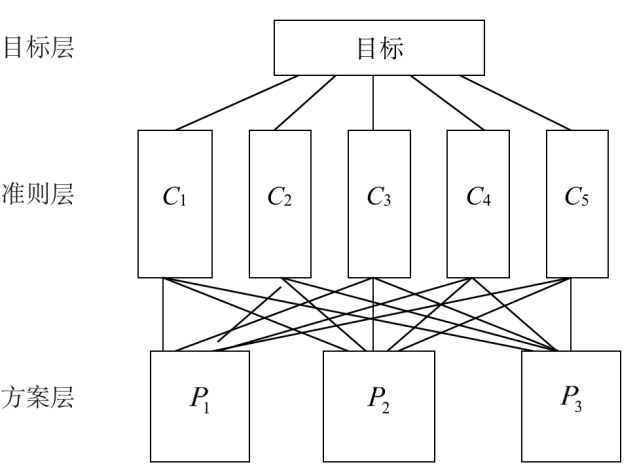
\includegraphics[height=0.25\textheight,width=0.5\linewidth]{figure/q1AHP}%宽度，源文件相对位置
	\caption{层次结构模型图}%图片下方的标题
	\label{fig:q1AHP}%图片引用时所需标签
\end{figure}

\subsubsection{构建层次分析模型}
\noindent \textbf{{\large 构建层次结构}}

首先，构建如下图所示的层次结构图，其中目标层为量化分析企业信贷风险，准则层为守约评分、经营规模、盈利能力、供应侧稳定性、需求侧稳定性、信誉评级六大因素，方案层为123家公司的信贷能力。

\begin{figure}[H]
	\centering
	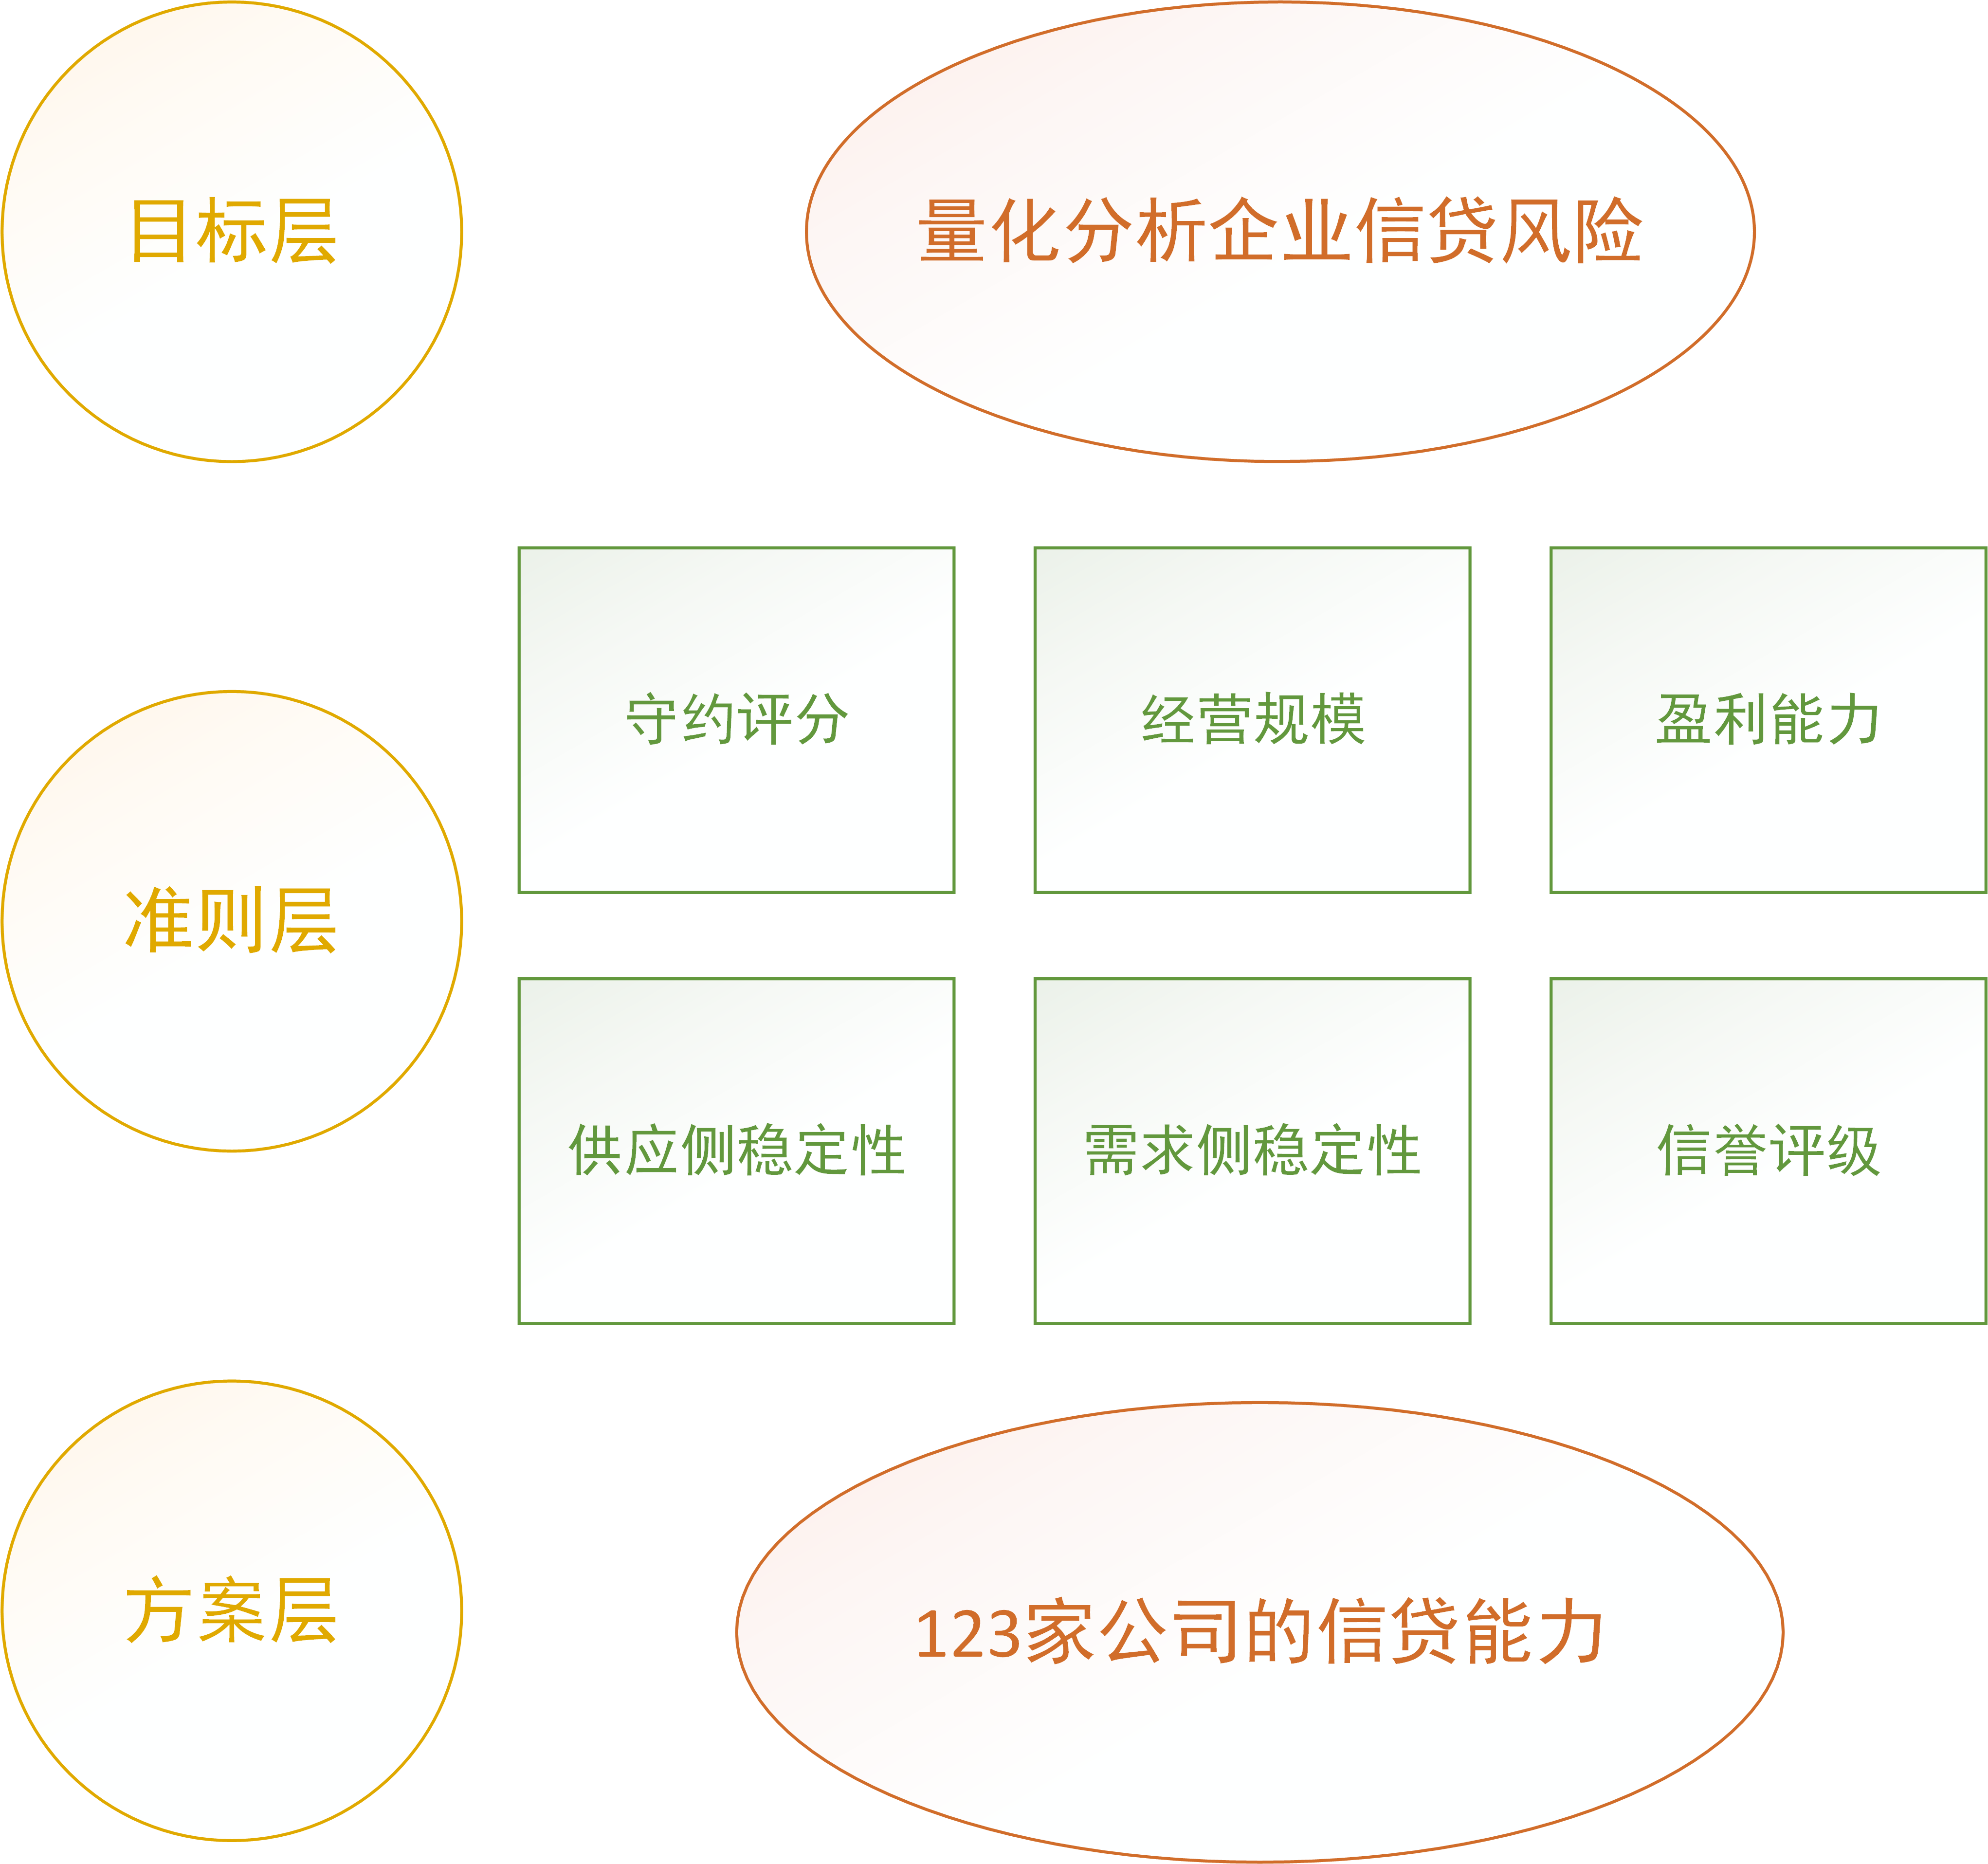
\includegraphics[height=0.25\textheight,width=0.5\linewidth]{figure/q1AHAModel}%宽度，源文件相对位置
	\caption{层次结构图}%图片下方的标题
	\label{fig:q1AHAModel}%图片引用时所需标签
\end{figure}

\noindent \textbf{{\large 构造成对比较矩阵}}

接着，我们通过比较六个因素两两之间相对重要程度，构造出目标层与准则层之间的成对比较矩阵。

\begin{tcolorbox}[breakable]
	\begin{verbatim}
		%目标层与准则层之间的成对比较矩阵
		A =[
		1  8  3  5  6  1; 
		1/8  1  1/7  1/5  1/4  1/8;
		1/3  7  1  3  2  1/3;
		1/5  5  1/3  1  1/3  1/5;
		1/6  4  1/2  3  1  1/4;
		1  8  3  5  4  1;];
	\end{verbatim}
\end{tcolorbox}

\subsubsection{求解层次分析模型}

我们在MATLAB中调用预先编写好的函数\verb|AHP()|，该函数的代码可以在附录中找到。

\begin{tcolorbox}[breakable]
	\begin{verbatim}
		[W, Lmax, CI, CR] = AHP(A)
	\end{verbatim}
\end{tcolorbox}

随后，我们得到如下所示对应的权重向量$ W $、最大特征值$ L_{max} $、一致性指标$ CI $以及一致性比率$ CR $，并通过$ CI $与$ CR $，对所得出的权重向量，进行一致性检验，判断出该权重向量可作为最终的决策依据。

\[\left\{ \begin{array}{l}
		W = {[0.3482;0.0263;0.1475;0.0645;0.0952;0.3182]^{\rm{T}}} \\
		{L_{max}} = 6.3584                                         \\
		CI = 0.0717                                                \\
		CR = 0.0578
	\end{array} \right.\]

应用该权重向量，我们可以计算得出每个企业的信贷能力，如下图所示：

\begin{figure}[H]
	\centering
	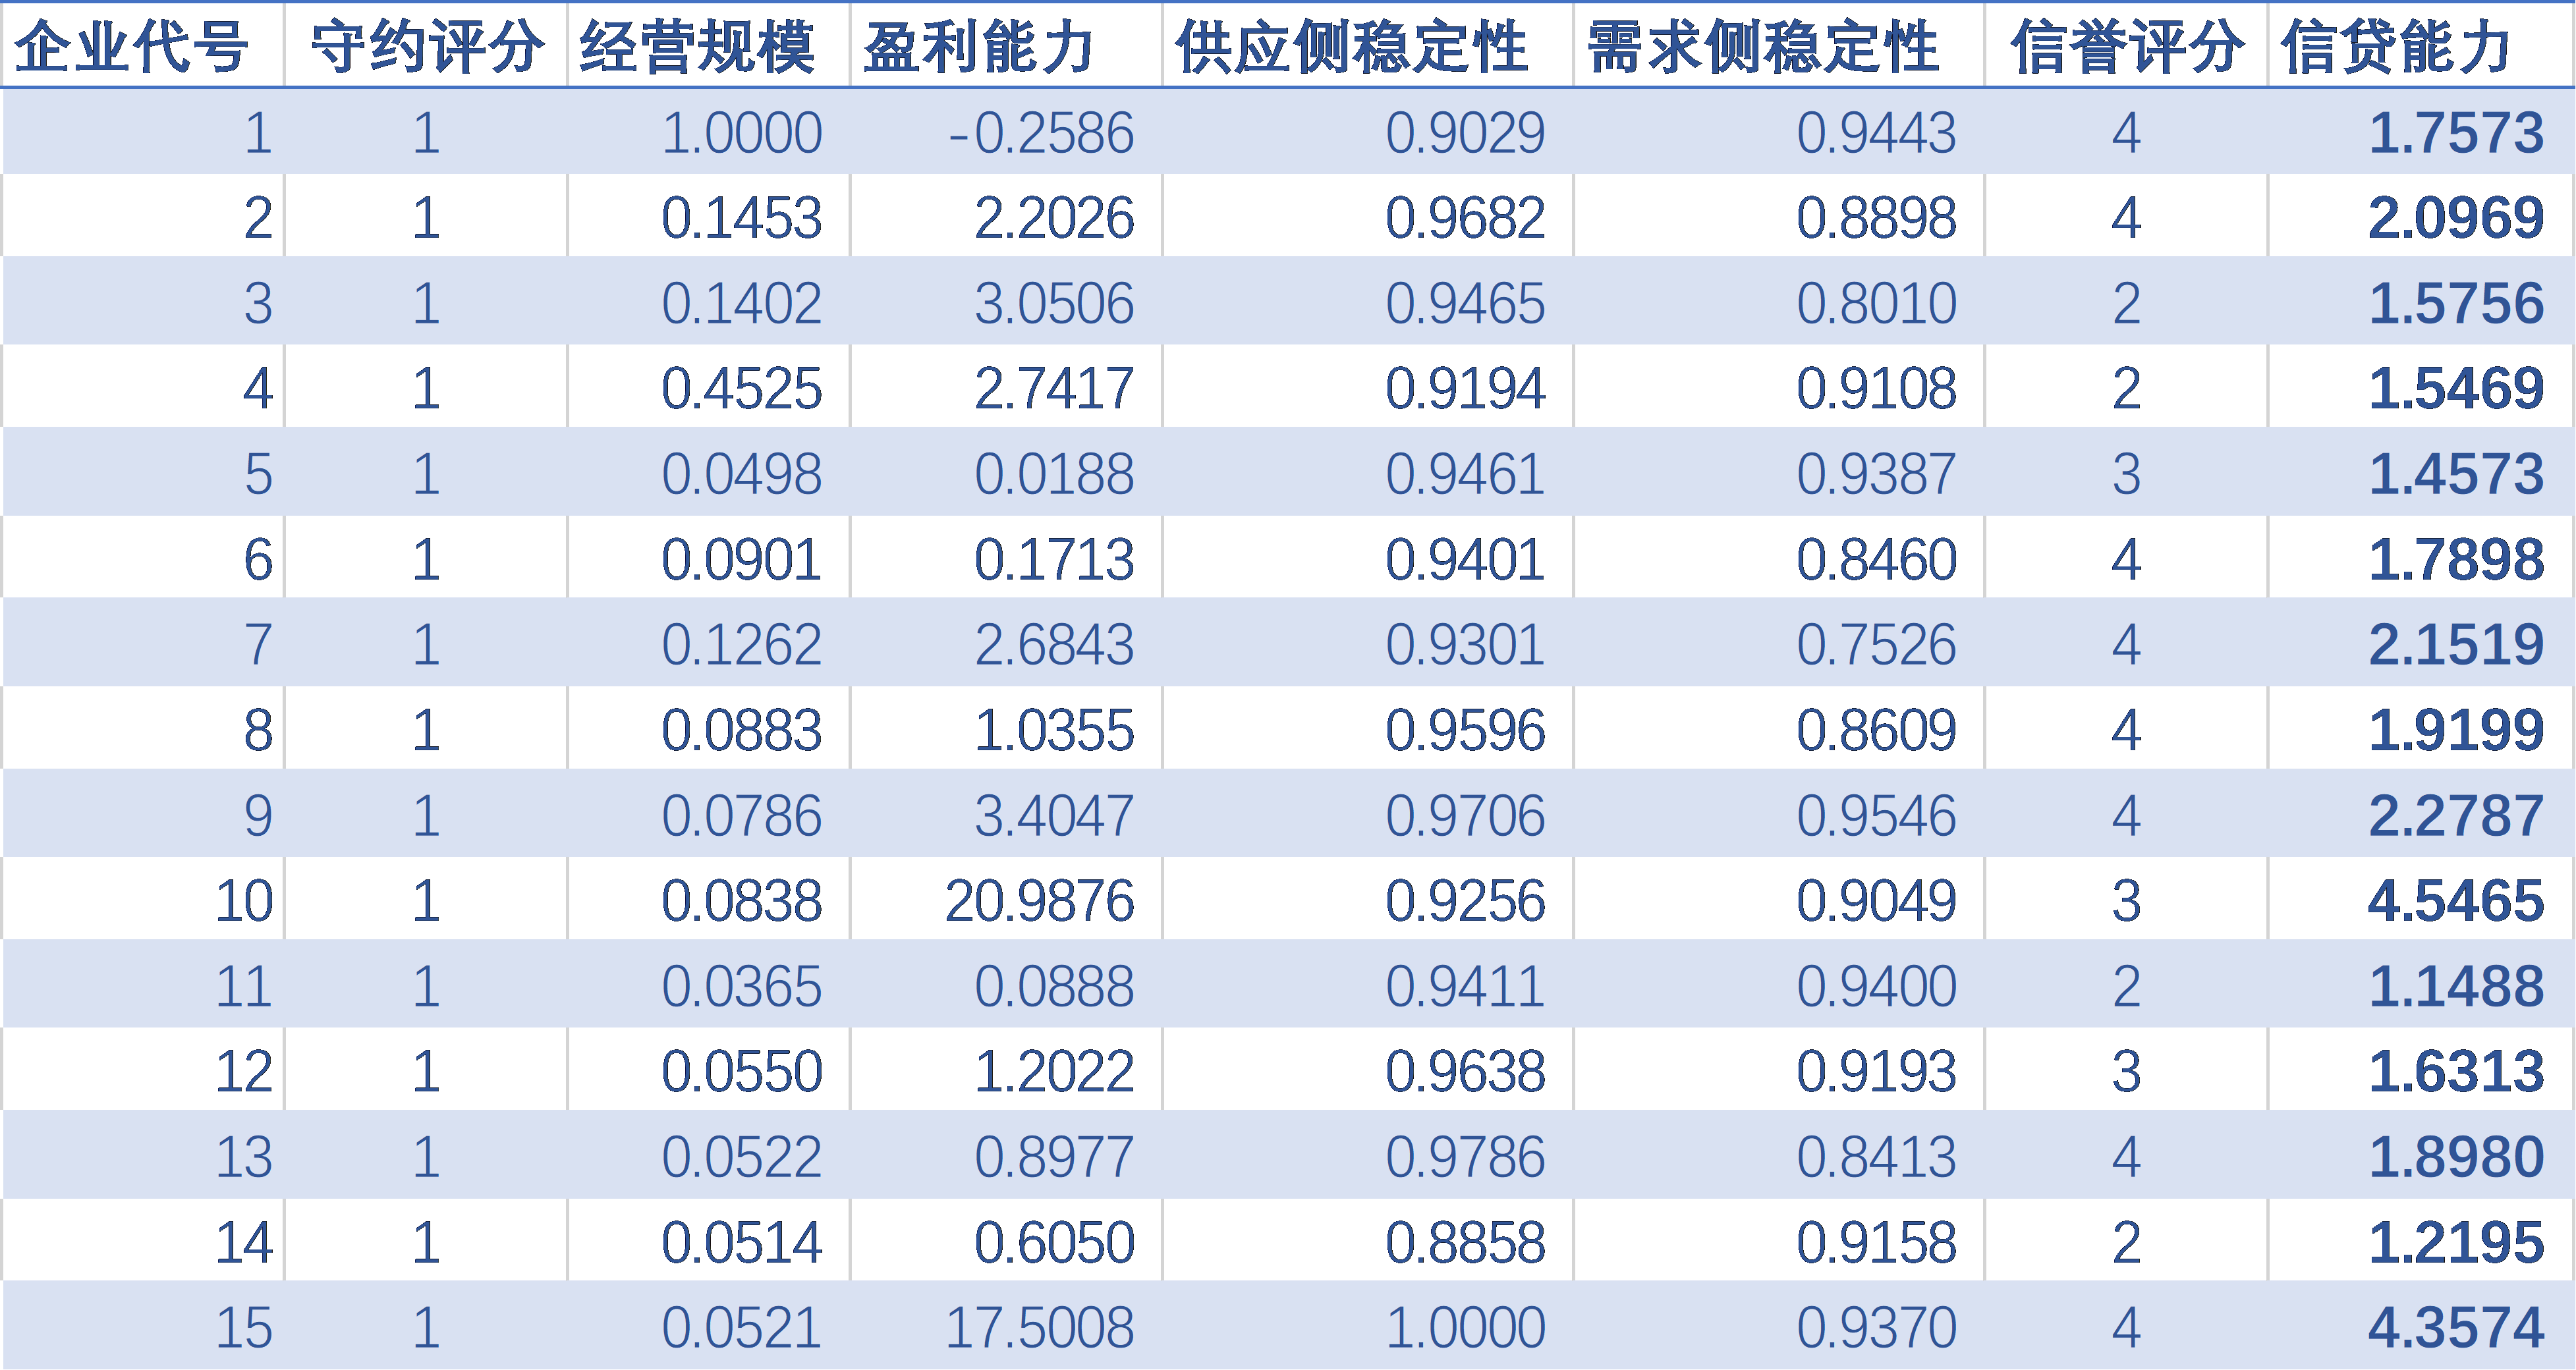
\includegraphics[width=0.5\linewidth]{figure/q1Ability}%宽度，源文件相对位置
	\caption{前15家企业的信贷能力}%图片下方的标题
	\label{fig:q1Ability}%图片引用时所需标签
\end{figure}


\subsubsection{层次分析模型的评价}

通过运用层次分析法，在构造出成对比较矩阵后，调用MATLAB中调用预先编写好的函数，分别计算出对应的权重向量$ W $、最大特征值$ L_{max} $、一致性指标$ CI $，一致性比率$ CR $。

权重向量$ W $，其权系数大小代表相应目标在多目标最优化问题中的重要程度，其值越大表示相应目标在问题中越重要。

最大特征值$ L_{max} $，以此来计算对应的一致性指标$ CI $、一致性比率$ CR $。

一致性指标$ CI $ ，当$ CI = 0 $，有完全的一致性；$ CI $接近于0，有满意的一致性；$ CI $越大，不一致越严重。

一致性比率$ CR $，若$ CR < 0.1 $，认为A的不一致程度在容许范围之内，否则应重新构造成对比较矩阵。

根据上述我们计算所得的结果显示，$ CR < 0.1 $，构造出的成对比较矩阵的不一致程度在容许范围之内，因此认为整个层次的比较判断通过一致性检验，可用上述所得特征向量作为权向量，可按组合权向量表示的结果进行决策。


\subsection{规划求解信贷策略}
\subsubsection{规划求解理论}

在信贷策略模型的建立方面，我们采用了规划求解理论\cite{ref1}以此建立数学模型。在现有的约束条件下，如何充分利用资源，使任务或目标完成得最好。或是在给定目标下，如何以最少的资源消耗，实现这个目标，这便是规划求解理论的主要内容。因此，我们需要根据以下三个步骤建立我们需要的模型：

\begin{enumerate}[1.]
	\item 根据影响所要达到目的的因素找到决策变量；
	\item 由决策变量和所在达到目的之间的函数关系确定目标函数；
	\item 由决策变量所受的限制条件确定决策变量所要满足的约束条件。
\end{enumerate}

\subsubsection{规划模型的构建}

下面是我们根据规划求解理论建立的信贷策略模型。在银行年度信贷总额固定并且每家企业贷款总额之和小于等于银行年度信贷总额的约束条件之下，我们需要使得银行收入的数学期望值达到最高，即可给出该银行在年度信贷总额固定时对这些企业的信贷策略。

在年利率不低于4\%并且不超过15\%，银行给予每家企业贷款额度不低于10万元并且不超过100万元的前提下，我们借助前述所分析出来的数据、信誉评级评分和信贷能力，结合企业的排位百分比，区分银行是否给企业贷款，并将可以贷款的企业的贷款额度和贷款年利率进行分档处理，共分为如下图所示的31种档位。在此分档面板中，我们通过排位百分比，将处于不同档位的企业的贷款额度、贷款年利率作出相应调整，使得实力越强，信誉越高的企业，即所处档位越前的企业，能够获得越大的贷款额度，但不超过100万元，越低的贷款年利率，但不低于4\%，以此达到向实力强、供求关系稳定的企业提供贷款，并对信誉高、信贷风险小的企业给予利率优惠的目的，从而使银行所获收入的数学期望值越高。

\begin{figure}[H]
	\centering
	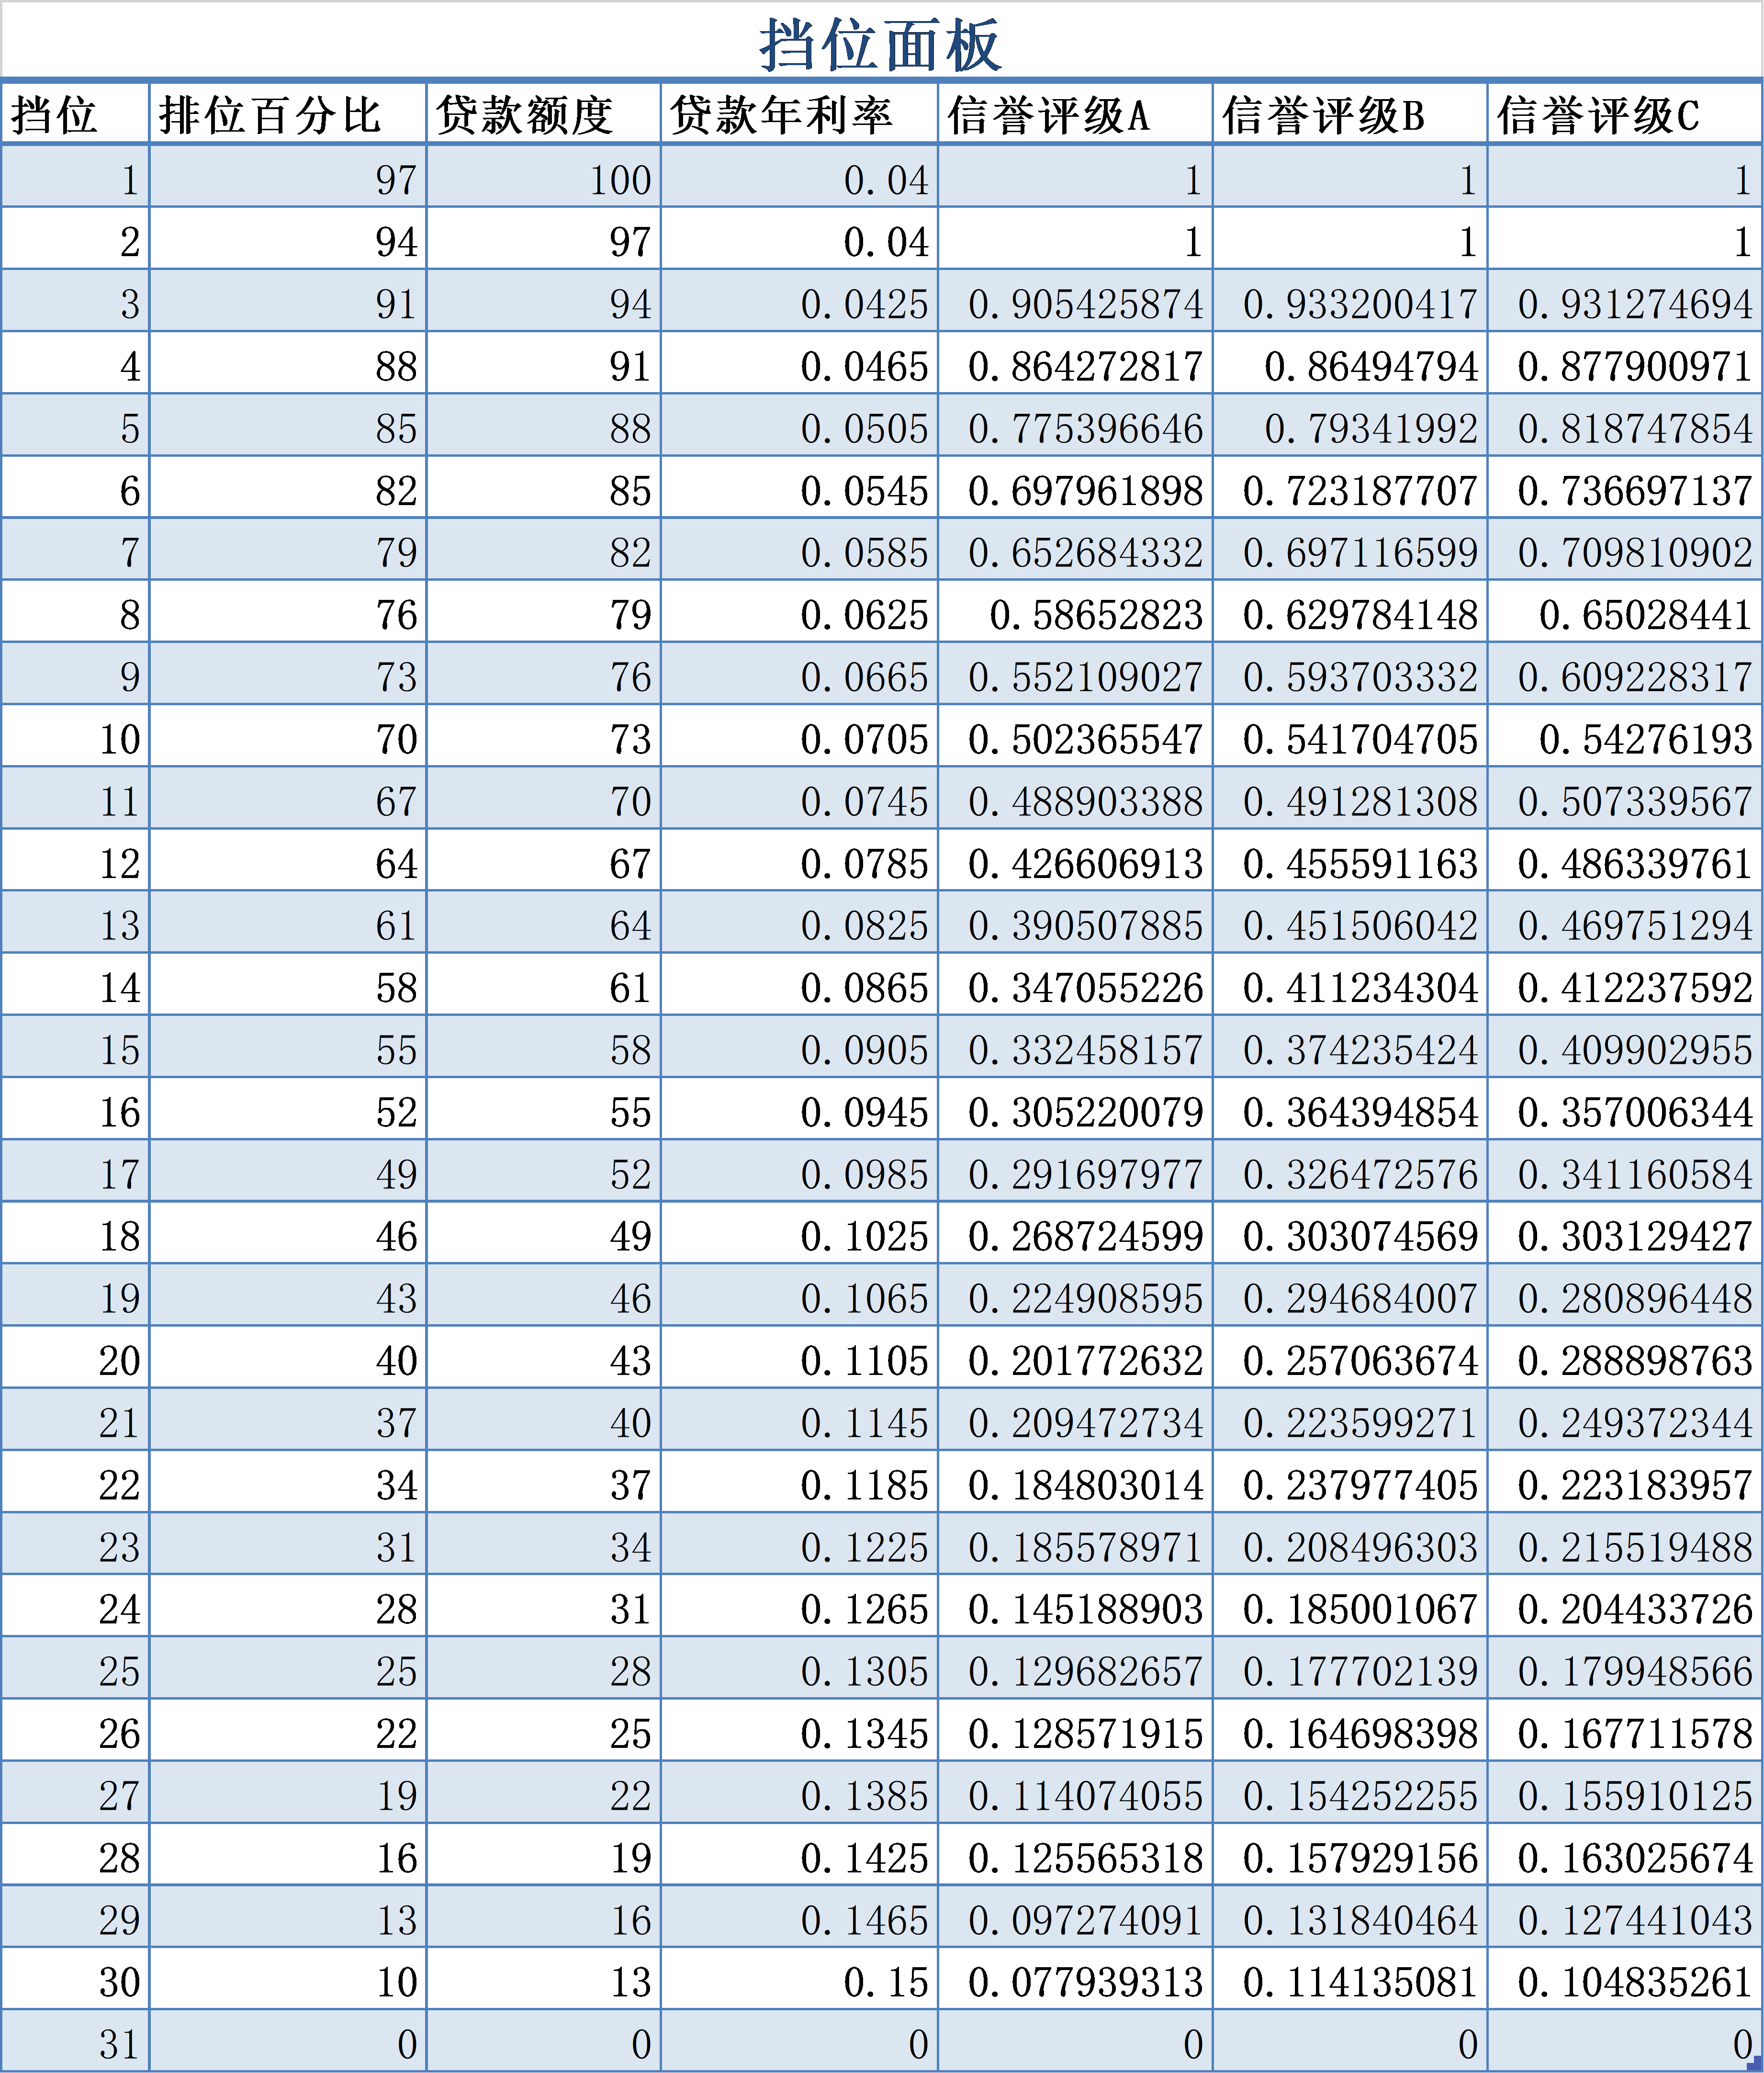
\includegraphics[width=0.5\linewidth]{figure/q1GearPanel}%宽度，源文件相对位置
	\caption{档位面板}%图片下方的标题
	\label{fig:q1GearPanel}%图片引用时所需标签
\end{figure}


\subsubsection{规划模型的求解}

当将企业的贷款额度及年利率加以分档之后，我们借助在MATLAB中预先编写好的代码，导入计算出的企业相关数据，进行相应处理后，调用函数\verb|linprog()|，具体代码可在附录中查看，最后得出在银行年度信贷总额固定时各家企业实际贷款额度。

下面展示随银行信贷总额变化时，部分企业贷款额度的变化数据：

\begin{figure}[H]
	\centering
	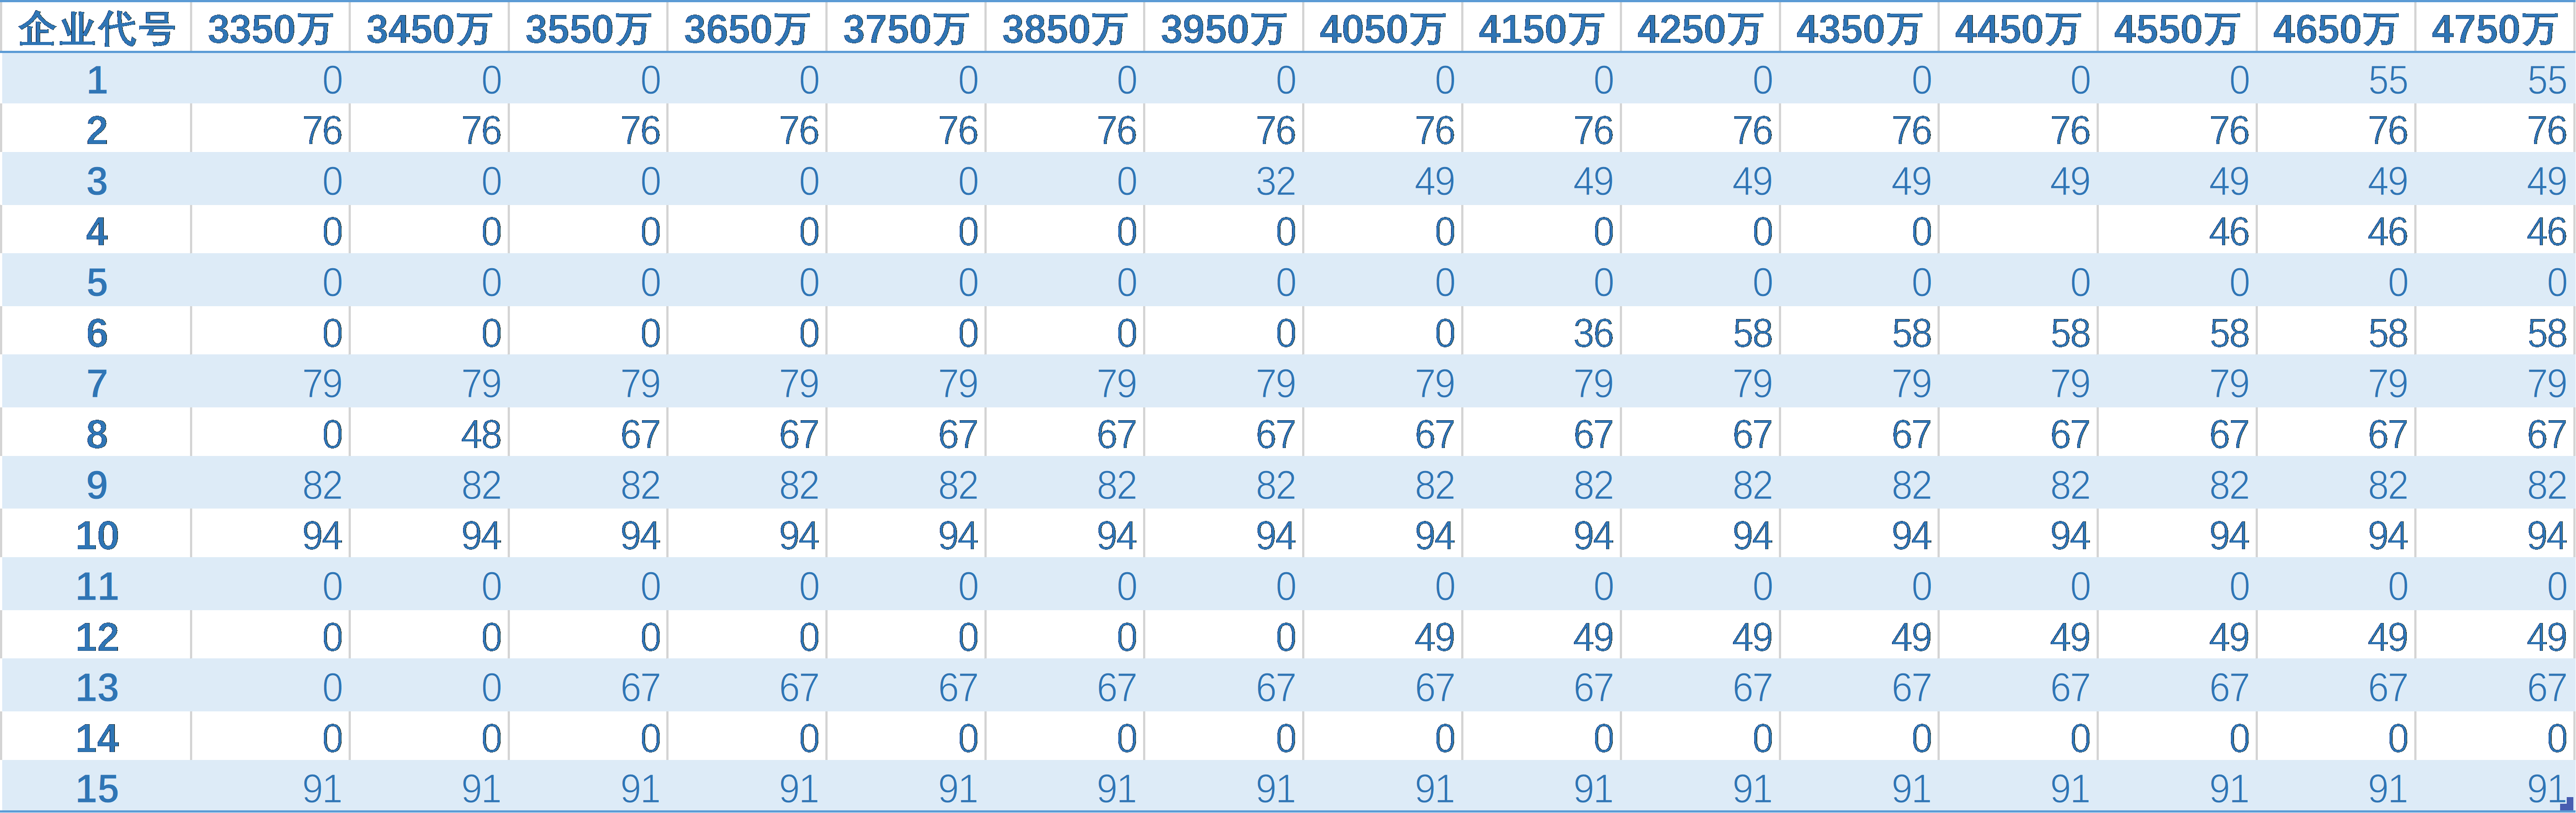
\includegraphics[width=0.75\linewidth]{figure/q1Table}%宽度，源文件相对位置
	\caption{规划求解部分结果}%图片下方的标题
	\label{fig:q1Table}%图片引用时所需标签
\end{figure}

%分文件结束
\ifx\allfiles\undefined
\end{document}
\fi